\documentclass[11pt]{beamer}
\usetheme{Pittsburgh}
\usepackage[utf8]{inputenc}
\usepackage[english]{babel}
\usepackage{amsmath}
\usepackage{amsfonts}
\usepackage{amssymb}
\usepackage{graphicx}

\usepackage{parcolumns}
\usepackage{siunitx}

\usepackage{pstricks}
\usepackage{pst-optexp}
\usepackage{xkeyval}

\author{Davide Bazzanella}
\title{Multidimensional Imaging of Ultrafast Laser Pulses}
%\setbeamercovered{transparent} 
\setbeamertemplate{navigation symbols}{} 
\logo{
\includegraphics[height=0.8cm]{Imperial_2_Pantones.eps}\vspace{233pt}\hspace{264pt}} 
\institute{Imperial College London} 
\date{16$^{\mathrm{th}}$ March 2016} 
\subject{Ultrafast Metrology}

\defbeamertemplate*{title page}{customized}[1][]{
\vspace{24pt}
\begin{center}
	{
	\usebeamerfont{title}\insertinstitute}\par
	\vspace{24pt}
	{BSc 3rd Year Project}\par
	\vspace{12pt}
 	{\usebeamerfont{title}\usebeamercolor[fg]{title}\inserttitle}\par
	\vspace{24pt}
	{\usebeamerfont{date}\insertdate}\par
	\vspace{24pt}
	\begin{parcolumns}{3}
		\colchunk[1]{Assessor:\\ \textbf{John Tisch}}
		\colchunk[2]{Supervisor:\\ \textbf{Tobias Witting}}
		\colchunk[3]{Student:\\ \textbf{Davide Bazzanella}}
	\end{parcolumns}
\end{center}
}

\begin{document}

\begin{frame}
\titlepage
\end{frame}

\begin{frame}{Outline}
\tableofcontents
\end{frame}

\section{Introduction}
\begin{frame}{Introduction}
\textbf{Field of study}:\\
	ultrafast laser metrology
	
\vspace{15pt}
\textbf{Aim}:\\
	measure the 3D spatial profile of an ultrafast laser pulse

\vspace{15pt}
\textbf{Challenge}:\\
	short duration of laser pulses, down to few femtoseconds ($\SI{e-15}{\s}$)
	
\vspace{15pt}
\textbf{Method}:\\
	direct measurement of single pulse is impossible,\\
	indirect approches measure the intensity averaged on many pulses
\end{frame}

\begin{frame}
\textbf{Techniques availables}:\\
\begin{itemize}
\item Spectrography
	\begin{itemize}
		\item Frequency-Resolved Optical Gating (FROG and variations)
	\end{itemize}
\item Interferometry
	\begin{itemize}
		\item Autocorrelation
		\item Spectral Phase Interferometry for Direct Electric field Reconstruction (SPIDER and variations).
	\end{itemize}
	\item Tomography
\end{itemize}

\vspace{15pt}
\textbf{Note}:\\
Normally, characterisation of a single spatial point in time (1D).\\
Can be extended to comprehend up to one spatial dimension (2D).
\end{frame}

\section{Fourier-Transform Spectral Interferometry}
\begin{frame}{Fourier-Transform Spectral Interferometry}
\textbf{Technique choosen}:\\
Mix of interferometric techniques.
Fourier-Transform Spectral Interferometry (FTSI) combined with a Mach-Zender interferometer and a SEA-F-SPIDER.\\
\begin{itemize}
	\item the MZ interferometer retrieves $I(\tau) 	= \int|U(t) + U_r(t)|^2\mathrm{d}t$
	\item SEA-F-SPIDER characterise the reference pulse $U_r(\omega)$
	\item FTSI obtains the time complex field through Fourier-transforms $U(\omega) \rightarrow U(\tau)$
\end{itemize}

\vspace{15pt}
\textbf{Our target}:\\
Obtain a full 3D characterisation of the laser pulse.
%
%\vspace{10pt}
%May be achieved with the use of a Mach-Zender interferometer
\end{frame}

%\begin{frame}
%describe the different steps of FTSI
%
%\begin{align}
%	I(\tau) 	&= \int|U(t)|^2\mathrm{d}t + \int|U_r(t)|^2\mathrm{d}t\\
%			&\quad + \int U(t)U_r^*(t-\tau)\mathrm{d}t + \int U^*(t)U_r(t-\tau)\mathrm{d}t 
%	\label{eq_inter}
%\end{align}
%
%\begin{align}
%	FT\left\lbrace I(\tau)\right\rbrace 	&= 	FT\left\lbrace \int|U(t)|^2\mathrm{d}t + \int|U_r(t)|^2\mathrm{d}t\right\rbrace \\
%			&\quad + \tilde{U}(\omega)\tilde{U}_r^*(\omega) + \tilde{U}^*(-\omega)\tilde{U}_r(-\omega)
%	\label{eq_fourier}
%\end{align}
%\begin{equation}
%\tilde{U}(\omega)\tilde{U}_r^*(\omega) = A(\omega) = |\tilde{U}(\omega)||\tilde{U}_r^*(\omega)|\mathrm{e}^{i[\psi(\omega)-\psi_r(\omega)]}
%\end{equation}
%\begin{equation}
%\tilde{U}(\omega)\mathrm{e}^{i\psi(\omega)} = \frac{A(\omega)}{|\tilde{U}_r^*(\omega)|}\mathrm{e}^{i\psi_r(\omega)}
%\end{equation}
%\end{frame}

\begin{frame}{Time complex field}
Start from:
\begin{align}
	I(\tau) 	&= I_p + I_r \nonumber\\
			&\quad+ \int U(t)U_r^*(t-\tau)\mathrm{d}t + \int U^*(t)U_r(t-\tau)\mathrm{d}t 
	\label{eq_inter}
\end{align}
Fourier-transform into the frequency domain:
\begin{align}
FT\left\lbrace I(\tau)\right\rbrace 	&= 	FT\left\lbrace I_p + I_r \right\rbrace \nonumber\\
&\quad+ \tilde{U}(\omega)\tilde{U}_r^*(\omega) + \tilde{U}^*(-\omega)\tilde{U}_r(-\omega)
	\label{eq_fourier}
\end{align}
\end{frame}
\begin{frame}
The complex field in the spectrum domain is:
\begin{equation}
\tilde{U}(\omega) = |\tilde{U}(\omega)|\mathrm{e}^{i\psi(\omega)} = \frac{A(\omega)}{|\tilde{U}_r(\omega)|}\mathrm{e}^{i\psi_r(\omega)}
	\label{eq_field_spectral}
\end{equation}
where $|\tilde{U}_r^*(\omega)|$ and $\psi_r(\omega)$ are the spectral intensity and phase given by the SPIDER.

\vspace{15pt}
It can be Fourier-transformed back into the time domain:
\begin{equation}
\tilde{U}(\tau) = \mathrm{FT}^{-1} \left\lbrace |\tilde{U}(\omega)|\mathrm{e}^{i\psi(\omega)} \right\rbrace
= \mathrm{FT}^{-1} \left\lbrace \frac{A(\omega)}{|\tilde{U}_r(\omega)|}\mathrm{e}^{i\psi_r(\omega)} \right\rbrace
	\label{eq_field}
\end{equation}
\end{frame}

\section{Setup}
\begin{frame}{Mach-Zender Interferometer}
	\begin{center}
		\begin{pspicture}(10,7)
			\pnodes(0,6){IN}(10,3){OUT}
			\pnodes(1,6){BSA}(5.5,3){BSB}
			\pnodes(1,1){C}(2.5,1){D}(2.5,3){E}(4.5,3){Focus}
			\pnodes(8,6){G}(8,4.5){H}(5.5,4.5){I}
			
			\addtopsstyle{OptComp}{mirrorwidth=1.5, mirrortype=extended}
			\addtopsstyle{OptComp}{bssize=1, bsstyle=plate}
			\addtopsstyle{Beam}{fillstyle=solid, fillcolor=red!50!white, linecolor=red, opacity=0.2}
			
			\beamsplitter(IN)(BSA)(C){BS1}
			
			\mirror(BSA)(C)(D){M1}
			\mirror(C)(D)(E){M2}
			\oapmirror[oapmirroraperture=1.3, mirrortype=extended](D)(E)(Focus){OAP}
			\pinhole[outerheight=1,innerheight=0.1,phlinewidth=0.1](Focus)(Focus){PH}
			
			\beamsplitter(I)(BSB)(OUT){BS2}
			
			\mirror(BSA)(G)(H){M3}
			\mirror(G)(H)(I){M4}
			\mirror(H)(I)(BSB){M5}
			
			\drawwidebeam[beamwidth=0.4](IN){1-6}(OUT)
			\drawwidebeam[beamwidth=0.4](IN)(BSA){7-9}{6}(OUT)
			
			\pnode(6,6){ND}
			\optbox[optboxsize=0.2 1.3, labeloffset=1](BSA)(ND){ND filter}
			\optbox[optboxsize=1.6 3.1](7,5.25)(9.2,5.25)
			\rput[r](9.65,5.5){$\tau$\psline[arrows=<->](-0.65, -0.15)(0.35, -0.15)}
			\rput[r](7,6.5){moving platform}
			
			\rput[l](4.5,1.5){$\textbf{BS1-2}$ 50/50 beamsplitters}
			\rput[l](4.5,1.1){$\textbf{M1-5}$ mirrors}
			\rput[l](4.5,0.7){$\textbf{OAP}$ parabolic mirror}
			\rput[l](4.5,0.3){$\textbf{PH}$ $\SI{20}{\um}$ pinhole}
		\end{pspicture}
	\end{center}
\end{frame}

%\begin{frame}
%\textbf{Mach-Zender components}:\\
%\begin{itemize}
%	\item 2x broadband \textbf{beamsplitters} with AR coating (BS1, BS2)
%	\item 5x standard metal \textbf{mirrors} (M1, M2, M3, M4, M5)
%	\item 1x gold coated off-axis \textbf{parabolic mirror} (OAP)
%	\item 1x \SI{20}{\um} \textbf{pinhole} (PH)
%	\item 1x \textbf{moving platform} (Zaber attuator) with a \SI{0.047625}{\um} minimum step.
%\end{itemize}
%\end{frame}

\begin{frame}
\textbf{Sources}:\\
\begin{itemize}
	\item HeNe c.w. laser, $\lambda_{HeNe} = \SI{632.8}{\nm}$ - used for alignment
	\item Ti:S modelocked laser, producing \SI{30}{\fs} pulses compressed into \SI{3.7}{\fs} pulses through a hollow fiber and broadband chirped mirrors.
\end{itemize}
	
%	\vspace{5pt}
\textbf{Sensor}:\\
\begin{itemize}
	\item Allied Vision Guppy Pro F-503, Industrial CMOS camera (2588 $\times$ 1940 standard resolution)
\end{itemize}

\end{frame}

\section{Data Analysis}
\begin{frame}{Data Analysis}
\begin{columns}[T,onlytextwidth]
\column{.49\textwidth}
	\begin{enumerate}
		\vspace{5pt}
		\item acquire $I(x,y,\tau_i)$ for $i = 1,2,3,\ldots, N$
		\vspace{20pt}
		\item Fourier-transform to $$FT\left\lbrace I(x.,y.,\tau)\right\rbrace = \tilde{I}(x.,y.,\omega)$$% for every pixel $(x.,y.)$.
		\vspace{-5pt}
		\item isolate $\tilde{I}_{int}$, multiply phases
		\vspace{10pt}
		\item Fourier transform back to $$FT^{-1}\left\lbrace\tilde{I}_{int}(x.,y.,\omega)\right\rbrace = I_{p}(x.,y.,\tau)$$% for every pixel $(x.,y.)$.
	\end{enumerate}
\column{.49\textwidth}
	\begin{pspicture}(4,7)
		\psset{fillstyle=solid, fillcolor=white}
		\optbox[optboxsize=2 1](2.45,6.45)(3.45,6.45)
		\optbox[optboxsize=2 1](2.3,6.3)(3.3,6.3)
		\optbox[optboxsize=2 1](2.15,6.15)(3.15,6.15)
		\optbox[optboxsize=2 1](2,6)(3,6)
		\optdipole[labeloffset=1](2,6)(3,6){%
			\includegraphics[scale=.1]{imagesc2.eps}
		}
		\rput[r](1.4,6){$y$}
		\rput[r](2.6,5.3){$x$}
		\rput[r](4,5.6){$\tau$}		
		
		\optbox[optboxsize=2 1](2.45,4.45)(3.45,4.45)
		\optbox[optboxsize=2 1](2.3,4.3)(3.3,4.3)
		\optbox[optboxsize=2 1](2.15,4.15)(3.15,4.15)
		\optbox[optboxsize=2 1](2,4)(3,4)
		\rput[r](1.4,4){$y$}
		\rput[r](2.6,3.3){$x$}
		\rput[r](4,3.6){$\omega$}
		
		\optbox[optboxsize=2 1](2,2.5)(3,2.5)
		\rput[r](1.4,2.5){$I$}
		\rput[r](2.6,1.8){$\omega$}
	
		\optbox[optboxsize=2 1](2.45,0.95)(3.45,0.95)
		\optbox[optboxsize=2 1](2.3,0.8)(3.3,0.8)
		\optbox[optboxsize=2 1](2.15,0.65)(3.15,0.65)
		\optbox[optboxsize=2 1](2,0.5)(3,0.5)
		\rput[r](1.4,0.5){$y$}
		\rput[r](2.6,-0.2){$x$}
		\rput[r](4,0.1){$\tau$}
	\end{pspicture}
\end{columns}
\end{frame}

\begin{frame}{Interferogram}
\vspace{-15pt}
\begin{figure}
	\centering
	\includegraphics[scale=0.6]{interference2.eps}
\end{figure}
\vspace{-15pt}
\begin{equation*}
	I(\tau) 	= I_p + I_r + \int U(t)U_r^*(t-\tau)\mathrm{d}t + \int U^*(t)U_r(t-\tau)\mathrm{d}t 
\end{equation*}
\end{frame}

\begin{frame}{Spectrum and Phase}
\vspace{-15pt}
\begin{figure}
	\centering
	\includegraphics[scale=0.6]{spectrum_phase2.eps}
\end{figure}
\vspace{-5pt}
\begin{equation*}
FT\left\lbrace I(\tau)\right\rbrace 	= 	FT\left\lbrace I_p + I_r \right\rbrace 
+ \tilde{U}(\omega)\tilde{U}_r^*(\omega) + \tilde{U}^*(-\omega)\tilde{U}_r(-\omega)
\end{equation*}
\end{frame}

%\begin{frame}{Spectrum}
%\vspace{-15pt}
%\begin{figure}
%	\centering
%	\includegraphics[scale=0.6]{spectrum_zoom.eps}
%\end{figure}
%\vspace{-5pt}
%\begin{equation}
%\tilde{U}(\omega)\tilde{U}_r^*(\omega) = A(\omega) = |\tilde{U}(\omega)||\tilde{U}_r(\omega)|\mathrm{e}^{i[\psi(\omega)-\psi_r(\omega)]}
%	\label{eq_gauss}
%\end{equation}
%\end{frame}

%\begin{frame}
%\begin{enumerate}
%	\item acquire interferogram for each pixel at different delays
%\end{enumerate}
%\begin{figure}
%	\includegraphics[scale=0.6]{imagesc2.eps}
%\end{figure}
%\end{frame}

\begin{frame}
\begin{figure}
	\includegraphics[scale=0.6]{gaussian_filter.eps}
\end{figure}
\begin{equation}
\tilde{U}(\omega)\tilde{U}_r^*(\omega) = A(\omega) = |\tilde{U}(\omega)||\tilde{U}_r(\omega)|\mathrm{e}^{i[\psi(\omega)-\psi_r(\omega)]}
	\label{eq_gauss}
\end{equation}
\end{frame}

\begin{frame}{Spectrum and Phase}
\vspace{-15pt}
\begin{figure}
	\centering
	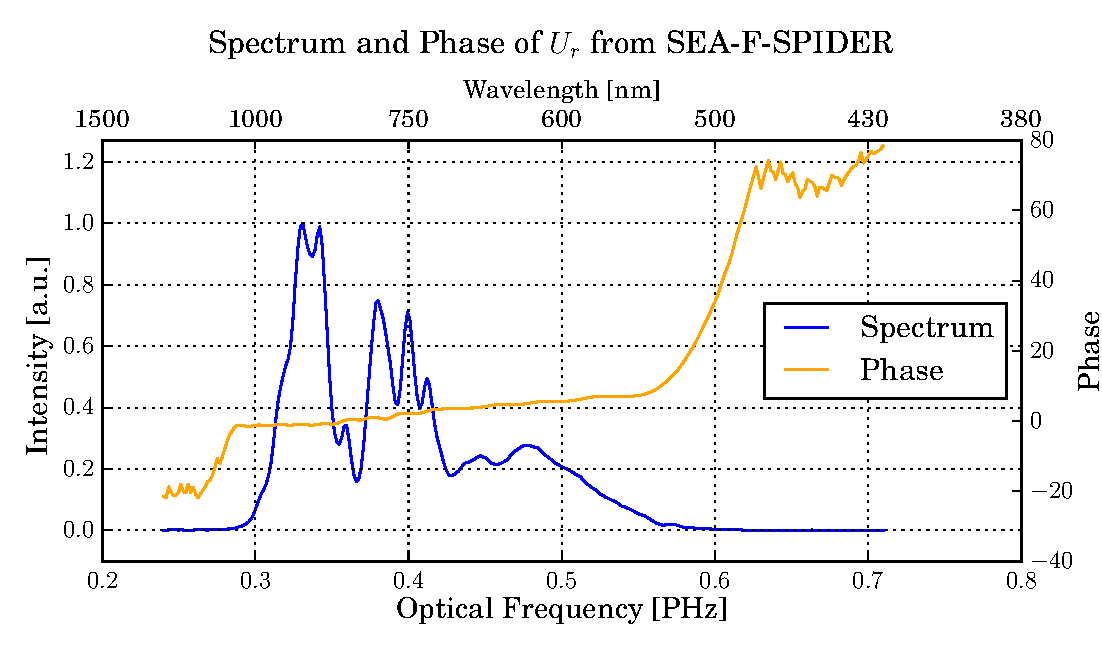
\includegraphics[scale=0.6]{spider_spectrum_phase.eps}
\end{figure}
\vspace{-5pt}
\begin{equation*}
\tilde{U}(\omega) = \frac{A(\omega)}{|\tilde{U}_r(\omega)|}\mathrm{e}^{i\psi_r(\omega)}
\end{equation*}
\end{frame}

\begin{frame}
\begin{figure}
	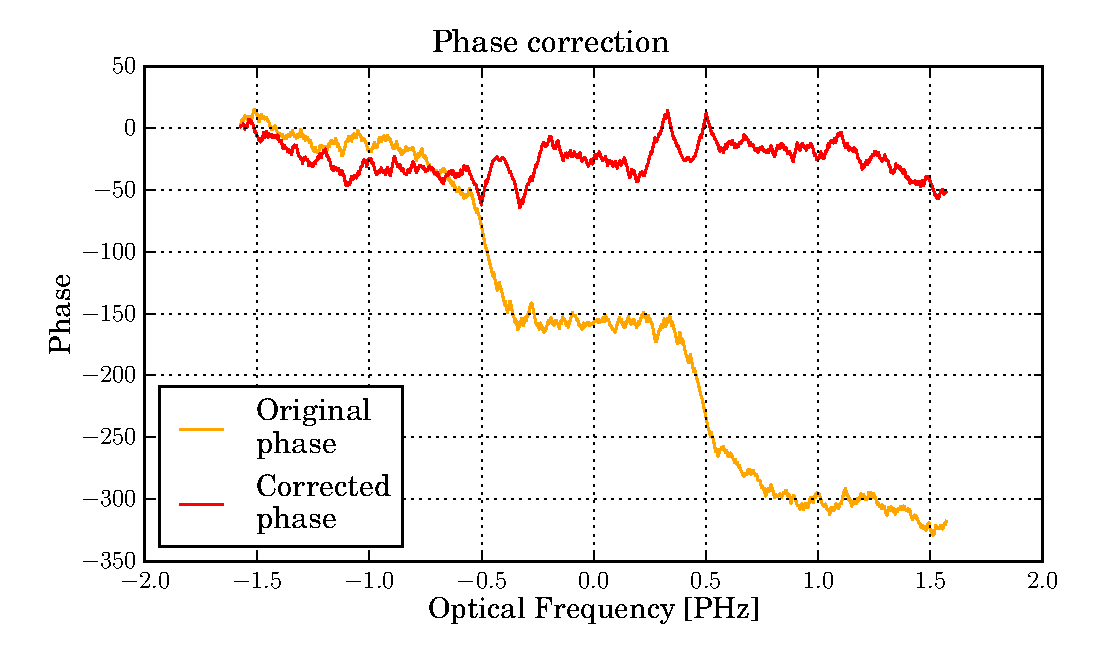
\includegraphics[scale=0.6]{phase_correction.eps}
\end{figure}
\begin{equation}
\Phi_{ND} = i\frac{\omega}{c}(\mathrm{n}_{ND}(\omega)-\mathrm{n}_{air})\mathrm{L}_{ND}
	\label{eq_ND_phase}
\end{equation}
\end{frame}

\begin{frame}{Paraboloid phase}
\begin{figure}
	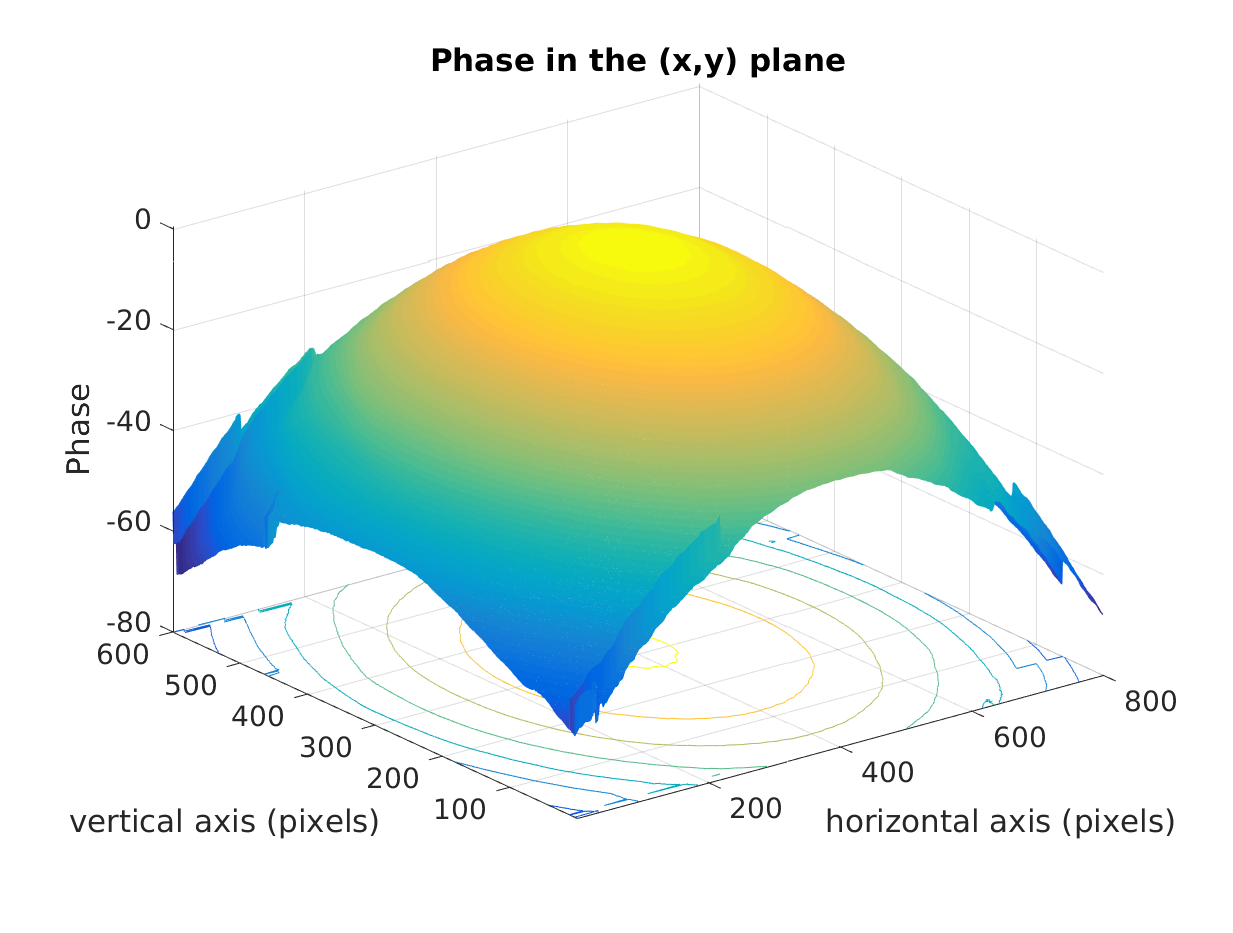
\includegraphics[scale=0.45]{phase2D.eps}
\end{figure}
\vspace{-15pt}
\begin{equation}
\phi = i\frac{\omega}{c}\frac{x^2 + y^2}{2\Delta z}
	\label{eq_paraboloid}
\end{equation}
\end{frame}

\section{Results and Conclusions}
\begin{frame}{Results}
\textbf{Results}:\\
	Phase correction does not work yet.

	\vspace{5pt}
\textbf{Improvements}:\\
	\begin{itemize}
		\item Use transparent glass to balance the arms
		\item Use 90/10 beamsplitter in place of 50/50 BS1
		\item Use of piezo stage for better sampling, but worse range
		\vspace{5pt}
		\item Use of corner cube retroreflectors (CCR) for better alignment
	\end{itemize}
	
%	\vspace{5pt}
%\textbf{Summary}:\\
	
\end{frame}
\begin{frame}{Conclusions}
Ultrafast laser metrology
\end{frame}
\end{document}
